\documentclass[conference]{IEEEtran}
\IEEEoverridecommandlockouts
% The preceding line is only needed to identify funding in the first footnote. If that is unneeded, please comment it out.
\usepackage{cite}
\usepackage{amsmath,amssymb,amsfonts}
\usepackage{algorithmic}
\usepackage{graphicx}
\usepackage{textcomp}
\usepackage{xcolor}
\def\BibTeX{{\rm B\kern-.05em{\sc i\kern-.025em b}\kern-.08em
    T\kern-.1667em\lower.7ex\hbox{E}\kern-.125emX}}
\begin{document}

\title{Detecting communities on social networks\\
}

\author{\IEEEauthorblockN{1\textsuperscript{st} Nguyen Hoang An}
    \IEEEauthorblockA{\textit{University of Information Technology} \\
        Ho Chi Minh City, Vietnamese \\
        20521051@gm.uit.edu.vn}
}

\maketitle

\begin{abstract}
    The report discusses a multi-layer clustering algorithm for community detection on social networks, specifically Twitter.
    This is a community clustering algorithm based on the similarity of structural components and content components, called MCT.
    From an application perspective, identifying such communities can provide better recommendations, along with other benefits.
\end{abstract}

\section{Introduction}
\begin{figure}[htbp]
    \centerline{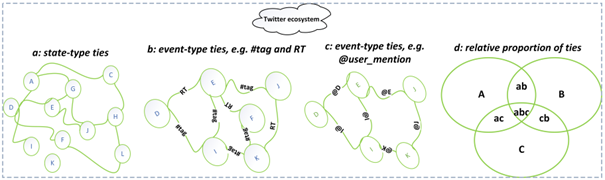
\includegraphics[scale=0.5]{fig1.png}}
    \caption{Types of interaction on Twitter.}
    \label{fig1}
\end{figure}

Today's social media networks like Twitter and Facebook are communities created by the diverse connections of countless users.
Consequently, this ecosystem is highly interconnected and forms various types of interactions, such as interactions among friends of friends, posts with tags, direct mentions @, or retweets on Twitter in Fig.~\ref{fig1}.
These interactions are what create communities on social media at different levels.

\section{Related Work}

\subsection{Graph-based and hierarchical methods}

Graph-based methods are algorithms that use graphs or network representations to model and analyze the structure of a system.
In these methods, nodes represent entities within the system, and edges represent the relationships between those entities.
Examples of graph-based methods include centrality measures, community detection algorithms, and network flow analysis.

Hierarchy-based methods are algorithms that organize data or systems into hierarchical structures, where smaller units are nested within larger units.
In these methods, the data or system is recursively partitioned into smaller and smaller units based on certain criteria, such as similarity or distance.
Examples of hierarchy-based methods include hierarchical clustering algorithms, decision trees, and nested sampling methods.

\subsection{Multiview and bi-modal clustering}

Multi-view clustering is an approach to clustering data that involves multiple representations or views of the same underlying dataset.
In this approach, each view represents a different aspect or feature of the data, and the goal is to integrate these views to determine a consensus clustering.
Multi-view clustering can be useful in cases of complex or high-dimensional data where different views can capture different aspects of the data.
Examples of multi-view clustering algorithms include Co-regularized Spectral Clustering and Multi-view K-Means.

Bi-modal clustering is a type of clustering algorithm that operates on data with two distinct modes or sources of information.
In this approach, the objective is to identify clusters that are consistent across both modes. Bi-modal clustering can be useful in cases where data has two separate but related sources of information, such as text and images, or gene expression and protein-protein interactions.
Examples of bi-modal clustering algorithms include Bi-Clustering and Coupled Bi-Clustering.

\section{Datasetss}
\subsection{Mental – Health Twitter}
This data was collected using the Twitter API.
The tweets have been filtered to retain only English contexts. It aims to classify users' mental health.
The dataset with fields such as post\_id, post\_created, post\_text, user\_id, followers, friends,favourites, statuses, retweets, label. Refer to Fig.~\ref{fig2}

\begin{figure}[htbp]
    \centerline{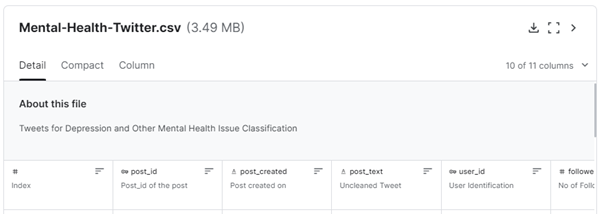
\includegraphics[scale=0.5]{fig2.png}}
    \caption{Mental – Health Twitter datasets}
    \label{fig2}
\end{figure}

\subsection{Tweets from US Capitol Riots}
This data was generated using the Twitter API + Tweepy. It consists of 80,000 tweets from January 6, 2021. The tweets have been stripped of mentions, hyperlinks, emojis, and punctuation. All text has been converted to lowercase.
The dataset with fields such as tweet\_id, text, query, user\_id, user\_name, follower\_count, user\_tweet\_count, likes, retweets, location\_name. Refer to Fig.~\ref{fig3}

\begin{figure}[htbp]
    \centerline{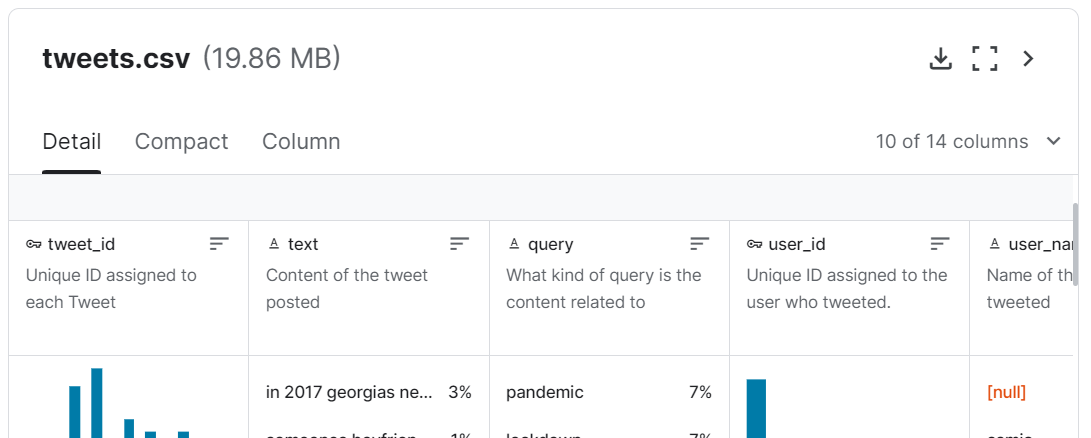
\includegraphics[scale=0.3]{fig3.png}}
    \caption{Tweets from US Capitol Riots datasets}
    \label{fig3}
\end{figure}

\section{Methodology}
The algorithm is defined through 3 stages.

Stage 1: Based on Dyadic Relationships - Bidirectional relationships between two nodes. Simmelian (Transitive) Relationships - Relationships between groups of at least 3 nodes, where there exist direct or indirect relationships between pairs of nodes to calculate the compatibility between node pairs using a algorithm in Fig.~\ref{fig5}.
The output of the algorithm is an n x n adjacency matrix representing the compatibility between nodes.
\begin{figure}[htbp]
    \centerline{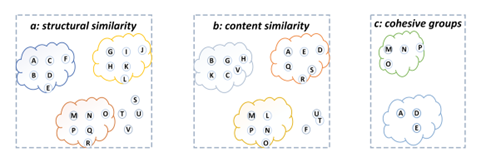
\includegraphics[scale=0.5]{fig4.png}}
    \caption{Node clustering in Detecting communities according to stages}
    \label{fig4}
\end{figure}

\begin{figure}[htbp]
    \centerline{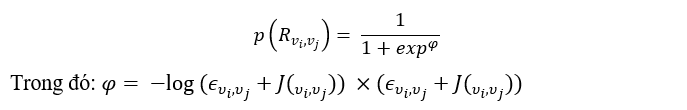
\includegraphics[scale=0.5]{fig5.png}}
    \caption{Algorithm for calculating compatibility between Node pairs}
    \label{fig5}
\end{figure}

Stage 2: We will convert the text components into individual vectors and apply the Latent Dirichlet Allocation (LDA) algorithm to identify a set of topics within the text corpus.
The distribution of topics for each tweet stream from related nodes is represented as a distribution of topics in the LDA model.
Next, we utilize the Jensen-Shannon distance (JSD) to measure the similarity between two probability distributions. This distance is symmetric and always has a finite value. The result returned is a similarity matrix of size m x m regarding content.

Stage 3: Apply clustering methods on both structural and textual aspects, then perform a function to combine the structural similarity matrix and the content similarity matrix to form an aggregate matrix.
Next, transform it into a distance matrix and cluster on this matrix until the stopping criteria are met.
The result of the algorithm is the clustered community
\section{Experiments}
Before proceeding with the main algorithm, we need to evaluate clustering algorithms for structural and content-based clustering.
\subsection{Structural}
The execution of the algorithm will produce two sets: Sr for structurally similar nodes and Su for structurally dissimilar nodes. The results are as depicted in the Fig.~\ref{fig7}.
\begin{figure}[htbp]
    \centerline{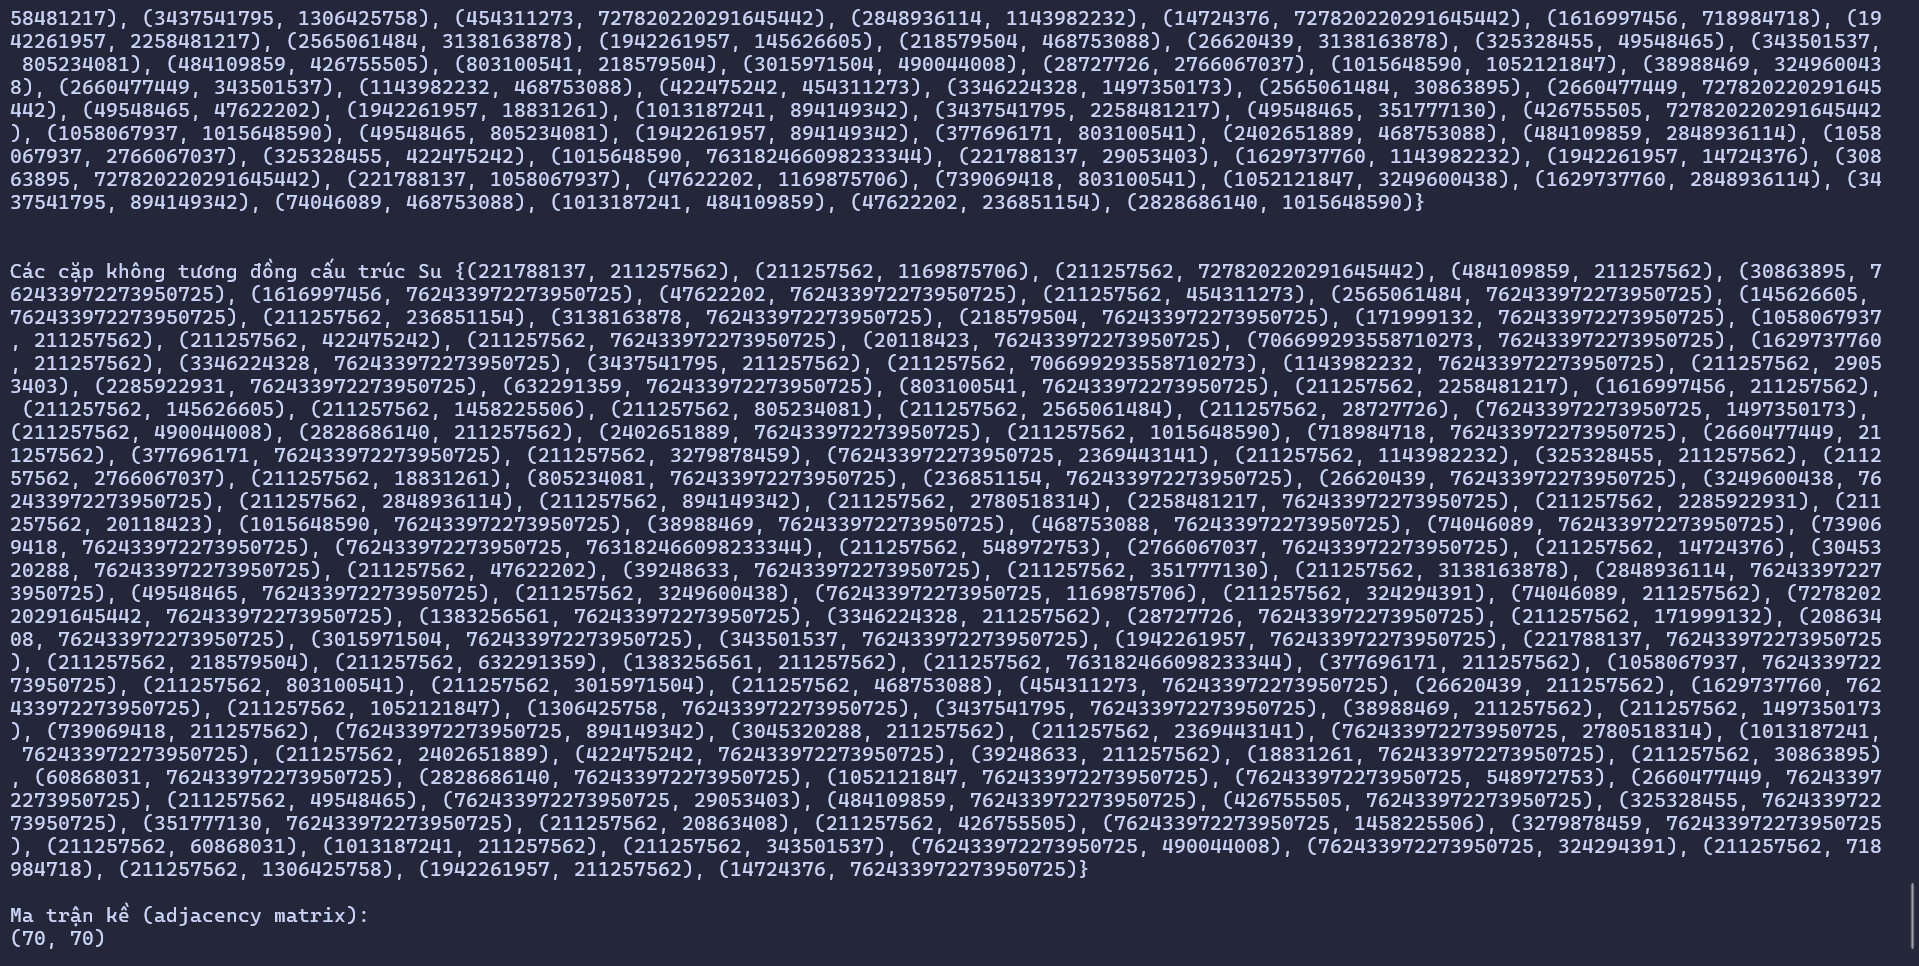
\includegraphics[scale=0.15]{fig7.png}}
    \caption{The results regarding structural similarity}
    \label{fig7}
\end{figure}
The structurally similar parts will be saved in the file 'Sr\_data\_with\_post\_text.csv' to serve as input data for the text similarity algorithm.

\subsection{Textual}

Similar to the structural similarity algorithm, this algorithm also generates two sets, Tr and Tu, corresponding to the sets of content similar and dissimilar nodes, respectively.
\begin{figure}[htbp]
    \centerline{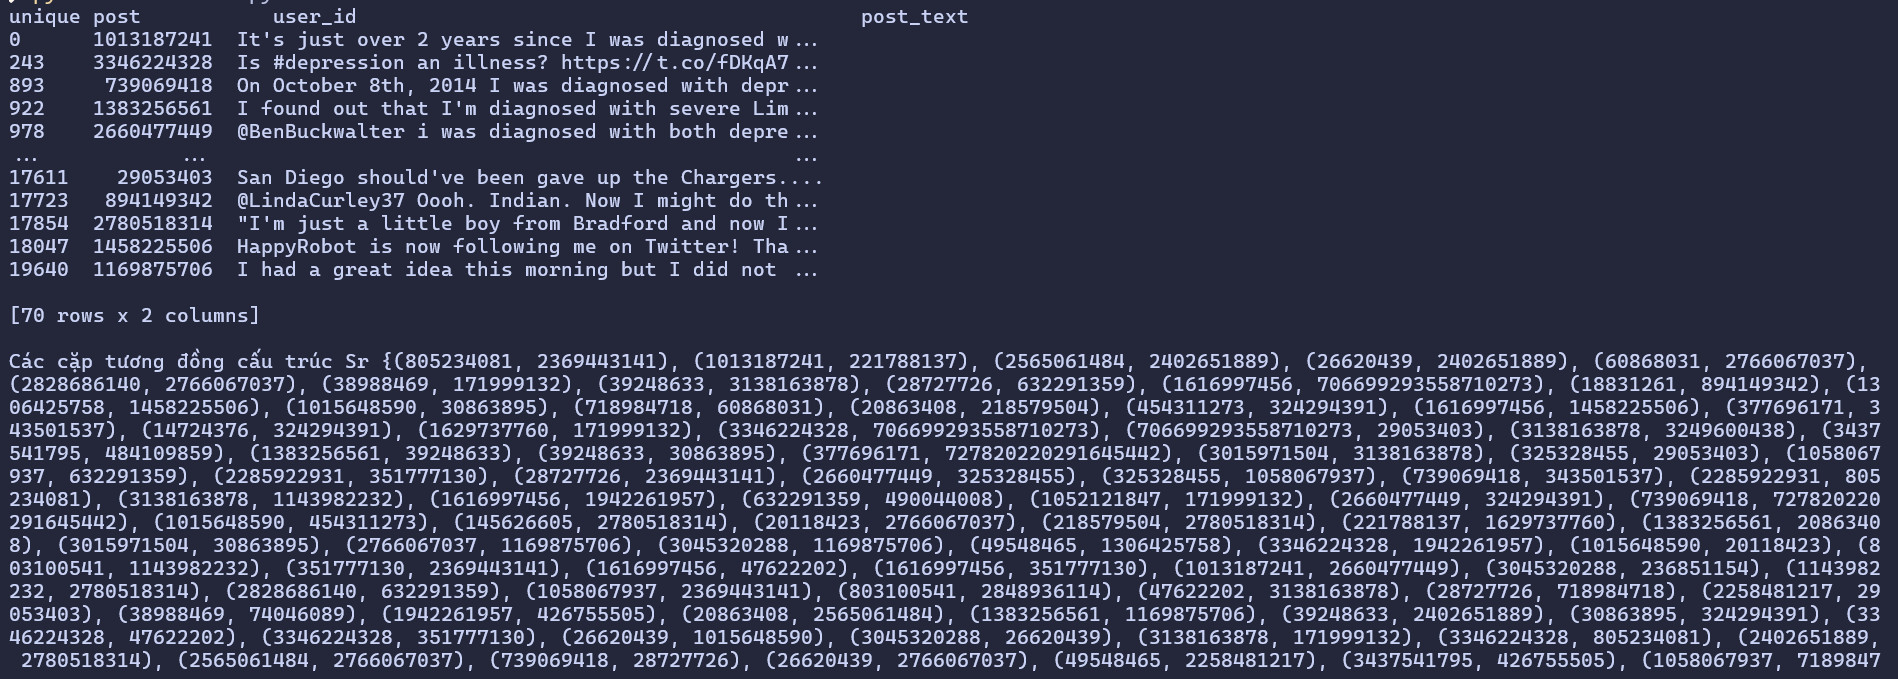
\includegraphics[scale=0.15]{fig8.png}}
    \caption{The results regarding textual similarity}
    \label{fig8}
\end{figure}
The result Fig.~\ref{fig8} is clusters of nodes with simple levels of structural and content similarity.
\subsection{Detecting communities}

\begin{figure}[htbp]
    \centerline{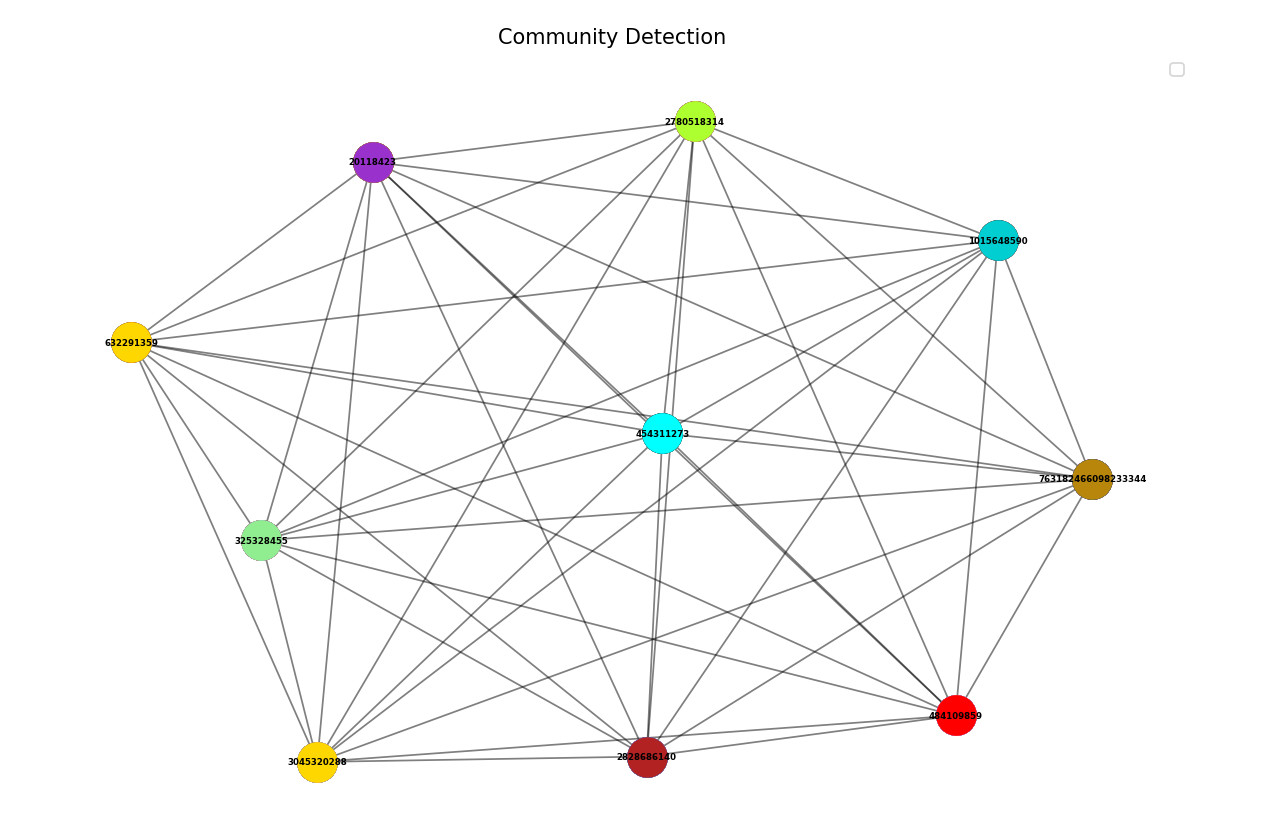
\includegraphics[scale=0.15]{fig6.png}}
    \caption{Clustering model with standard number of communities t = 10}
    \label{fig6}
\end{figure}

Perform clustering on the network data 'D' with a standard number of communities 't'.

Initialize functions like 'compute\_reciprocity\_prob', 'compute\_text\_similarity' , 'f\_structural', 'f\_textual' , 'compute\_pairwise\_similarities', 'detecting\_communities' to mine communities based on sample data.
Due to large data and not powerful personal computers, it leads to very long waiting times when taking large standard community numbers. For that reason, I do it with t = 10.

\section{Result Analysis}
The clustering method has demonstrated its ability to detect and identify highly cohesive communities within data.
In doing so, it not only helps address challenges stemming from incomplete data but also provides a comprehensive view of the community network.
Additionally, analyzing communities at multiple levels aids in a deeper understanding of the relationships and structures within each community.
This not only enhances the scalability of the method but also increases its flexibility when applied to various contexts and domains. This has proven to be quite beneficial for intelligent recommendation systems.

\section{Conclusion and Future Work}
Regarding the complexity of the proposed method, when the network size is large, the challenge lies in accurately determining when the algorithm for community detection will converge.
Therefore, the research team only uses one iteration to analyze the complexity of the algorithm, providing information on future performance. Assuming the execution complexity of a basic algorithm parameterized as f(C), the complexity of the algorithm will be approximately O(f(C) × s × r × m),
where s is the number of comparisons to decide the next cluster, r is the size, and m is the number of runs. In terms of execution, the complexity of the algorithm is relatively low; however, it tends to increase as the amount of data increases, thus requiring continued improvement in future work.

The complexity depends on the number of comparisons to decide the next cluster and the number of iterations to determine the optimal number of clusters.
So there is a need to research a method that can identify more intrinsic components accurately to minimize the number of comparisons as well as the number of iterations.
\begin{thebibliography}{9}
    \bibitem{Inuwa-Dutse2021}
    Isa Inuwa-Dutse, Mark Liptrott, Ioannis Korkontzelos.
    \textit{A multilevel clustering technique for community detection}.
    2021.

    \bibitem{Researchgate2019a}
    Researchgate.
    \textit{Simmelian Ties on Twitter: Empirical Analysis and Prediction}.
    2019.

    \bibitem{Researchgate2019b}
    Researchgate.
    \textit{Analysis and Prediction of Dyads in Twitter}.
    2019.

    \bibitem{Infamouscoder2022}
    Infamouscoder, Kaggle.
    \textit{Mental – Health Twitter datasets}.
    2022.
\end{thebibliography}
\end{document}